%
% ait.tex
%
% Copyright (C) 2021 by SpaceLab.
%
% Radio Occultation Documentation
%
% This work is licensed under the Creative Commons Attribution-ShareAlike 4.0
% International License. To view a copy of this license,
% visit http://creativecommons.org/licenses/by-sa/4.0/.
%

%
% \brief AIT campaign.
%
% \author Gabriel Mariano Marcelino <gabriel.mm8@gmail.com>
%
% \institution Universidade Federal de Santa Catarina (UFSC)
%
% \version 0.1.0
%
% \date 2021/03/02
%

\chapter{Assembly, Integration and Test} \label{ch:ait}

The following activities refer to the Flight Model, so after the execution of this AIT the CubeSat will not suffer any modification in its hardware, software, and firmware. The only acceptable interference is the recharge of batteries, which is made through an external umbilical cable.

In \autoref{fig:sequence} there is a general view of the sequential steps to the entire AIT campaign, where I refers to integration activities and T is used for testing activities.


%GOLDS is a space technology demonstration mission created by the \ac{UFSC}, Brazil. The main goal is to provide the service module for the Environmental Data Collector \ac{EDC} payload from INPE-RN. The service module was developed at UFSC and it has three main components: the Electric Power System \ac{EPS}, the On-Board Data Handling \ac{OBDH} and Telemetry, Tracking and Command \ac{TTC}.

%Besides performing the EDC main functionalities, the mission will contribute to validating key technologies that will enable faster and cheaper development of future satellites reusing the same core structure. As an educational mission, it also serves to train engineering students in space mission conception, design, implementation and operation in all areas involved. 

%It also acts as an experimenting platform for research in space technologies developed before, during, and after the operations phase of the mission, providing empirical data for experiments of many kinds. GOLDS is expected to be launched by the end of 2023.

\begin{figure}[!htb]
\centering
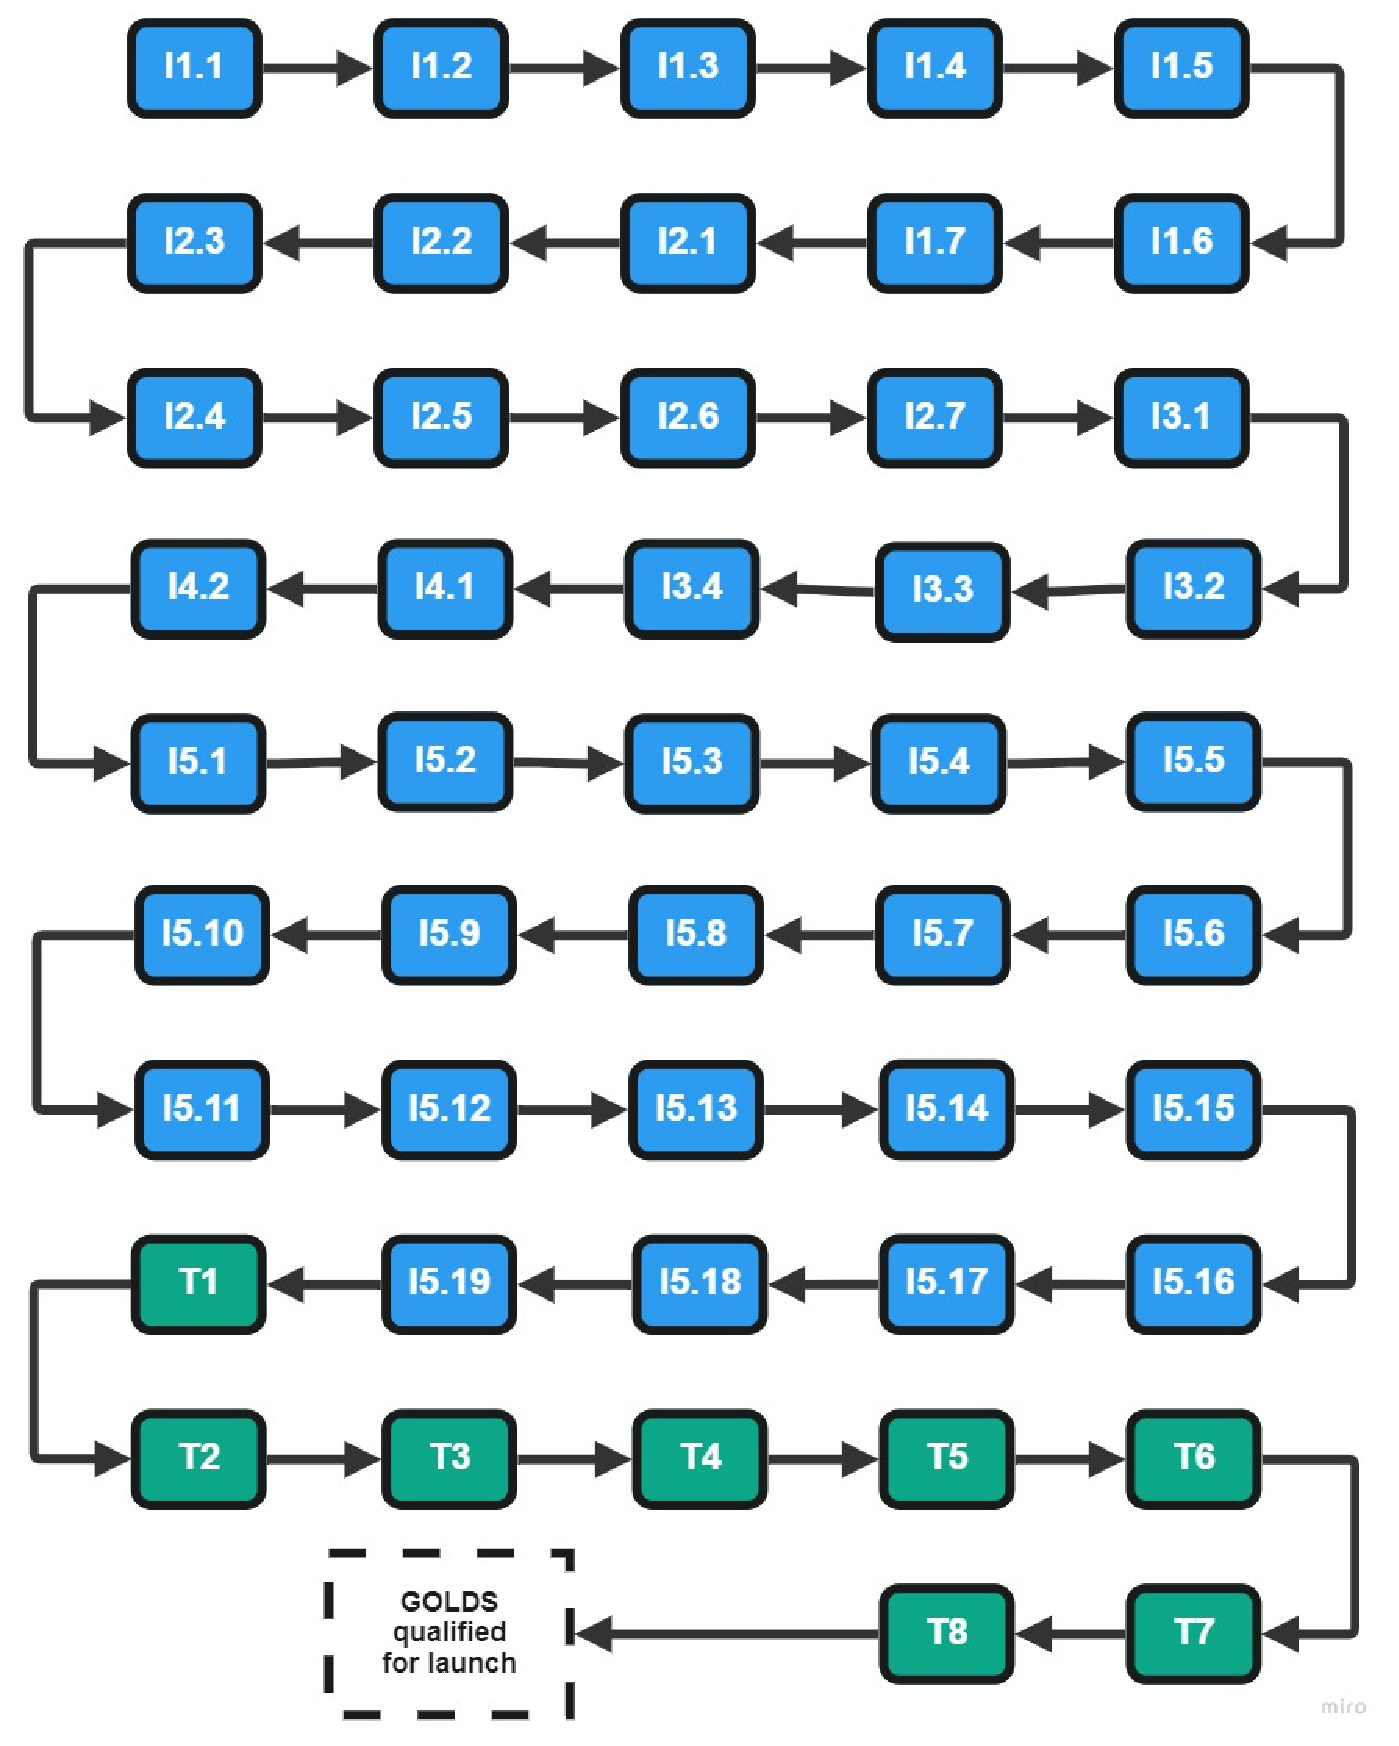
\includegraphics[scale=0.45]{figures/Assembly and Tests chart.pdf}
\caption{Sequence of activities of AIT plan.}
\label{fig:sequence}
\end{figure}

\section{Assembly Instructions}
Each task in the Integration segment of the AIT campaign is listed in Table \ref{table_integration} together with a label for the block, name and section with further details. %\The complete guideline of them are in Appendix ref{AppendixIntegration}.

%\subsection{Preparation and Required Material}

%\subsection{Assembly Steps}

\begin{table}[!htb]
\centering
\begin{tabular}{llc}
    \toprule[1.5pt]
 	\textbf{Block} & \textbf{Name} & \textbf{Section} \\
 	\midrule
    I1.2     & I1.2: To pre-mount battery+case and EPS                           & {I1} \\
	I1.3     & I1.3: I1.2+Bottom structure                                       & {I1} \\
    I1.4     & I1.4: I1.3+Primary OBDH                                           & {I1} \\
    I1.5     & I1.5: I1.4+Radiation Monitor                                      & {I1} \\
    I1.6     & I1.6: I1.5+Interface Module                                       & {I1} \\
    I1.7     & I1.7: I1.6+Top structure                                          & {I1} \\
    I2.1     & I2.1: To pre-mount upper (U) modules                              & {I2} \\
    I2.2     & I2.2: Interface Module+Bottom structure                           & {I2} \\
    I2.3     & I2.3: I2.2+Redudant EDC                                           & {I2} \\
    I2.4     & I2.4: I2.3+Primary EDC                                            & {I2} \\
    I2.5     & I2.5: I2.4+Radiation instrument                                              & {I2} \\
    I2.6     & I2.6: I2.5+TT\&C                                                  & {I2} \\
    I2.7     & I2.7: I2.6+Top structure                                          & {I2} \\
    I3.1     & I3.1: Debug interface (-X and +X)+Lateral structure               & {I3} \\
    I3.2     & I3.2: I3.1+ADCS+Lateral structure                                 & {I3} \\
    I3.3     & I3.3: I1.7+ADCS                                                   & {I3} \\
    I3.4     & I3.4: I2.7+Magnet+upper(U) top structure                          & {I3} \\
    I4.1     & I4.1: I1.7+I2.7+I3.5                                              & {I4} \\
	I1.1     & I1.1: To pre-mount lower (U) modules                              & {I4} \\
    I4.2     & I4.2: I4.1 and I4.2+Debug interface (-Y and +Y)+Lateral structure & {I4} \\
    I5.1     & I5.1: I4.2+Shield (-Z)                                            & {I5} \\
    I5.2     & I5.2: I5.1+Shield (Z0;X0)                                         & {I5} \\
    I5.3     & I5.3: I5.2+Shield (Z0;X1)                                         & {I5} \\
    I5.4     & I5.4: I5.3+Shield (Z0;Y0)                                         & {I5} \\
    I5.5     & I5.5: I5.4+Shield (Z0;Y1)                                         & {I5} \\
    I5.6     & I5.6: I5.5+Shield (Z1;X0)                                         & {I5} \\
    I5.7     & I5.7: I5.6+Shield (Z1;X1)                                         & {I5} \\
    I5.8     & I5.8: I5.7+Shield (Z1;Y0)                                         & {I5} \\
    I5.9     & I5.9: I5.8+Shield (Z1;Y1)                                         & {I5} \\
    I5.10    & I5.10: I5.9+Antenna+SP(+Z)                                        & {I5} \\
    I5.11    & I5.11: I5.10+SP (-Z)                                              & {I5} \\
    I5.12    & I5.12: I5.11+SP (Z0;X0)                                           & {I5} \\
    I5.13    & I5.13: I5.12+SP (Z0;X1)                                           & {I5} \\
    I5.14    & I5.14: I5.13+SP (Z0;Y0)                                           & {I5} \\
    I5.15    & I5.15: I5.14+SP (Z0;Y1)                                           & {I5} \\
    I5.16    & I5.16: I5.15+SP (Z1;X0)                                           & {I5} \\
    I5.17    & I5.17: I5.16+SP (Z1;X1)                                           & {I5} \\
    I5.18    & I5.18: I5.17+SP (Z1;Y0)                                           & {I5} \\
    I5.19    & I5.19: I5.18+SP (Z1;Y1)                                           & {I5} \\
    \bottomrule[1.5pt]
	\end{tabular}
    \caption{List of integration activities.}
    \label{table_integration}
\end{table}

\section{Environmental Testing}

After the integration, the tests that will be executed in the AIT campaign to qualify Radio Occultation for launch are in Table \ref{table_test}. Each of these tests receives the letter T and a number for identification. %Table \ref{table_test} brings the label of the block, name of test and section with further details of the respective test.

\begin{table}[!htb]
    \centering
    \begin{tabular}{lll}
        \toprule[1.5pt]
    	\textbf{Block} & \textbf{Name} & \textbf{Criteria} \\
    	\midrule
    	T1    & Dimensions                  & \parbox[t]{8cm}{Dimensions of 100.0 $\times$ 100.0 $\times$ 227.0 mm $\pm$0.1 mm in the X, Y, and Z axis} \\
        T2    & Fit check                   & \parbox[t]{8cm}{Absence of interference and a smooth sliding through the deployer} \\
    	T3    & Mass                        & Total CubeSat mass below or equal to 4.00 kg \\
    	T4    & Center of gravity           & \parbox[t]{8cm}{It must be within ±2.0 cm from the geometric center on the X-Axis and Y-Axis, and less than $\pm$4.5 cm in Z-axis} \\
        T5    & Vibration                   & To be defined by the launch vehicle \\
        T6    & Thermal cycling             & To be defined by the launch vehicle \\
        T7    & Thermal Vacuum Bake-out     & To be defined by the launch vehicle \\
        T8    & EMC testing                 & To be defined by the launch vehicle \\
        \bottomrule[1.5pt]
	\end{tabular}
    \caption{\label{table_test}List of qualifying tests and simulations.}
\end{table}

The sequence of these tests is summarized in Fig. \ref{fig:testesequency}.

\begin{figure}[!htb]
    \centering
    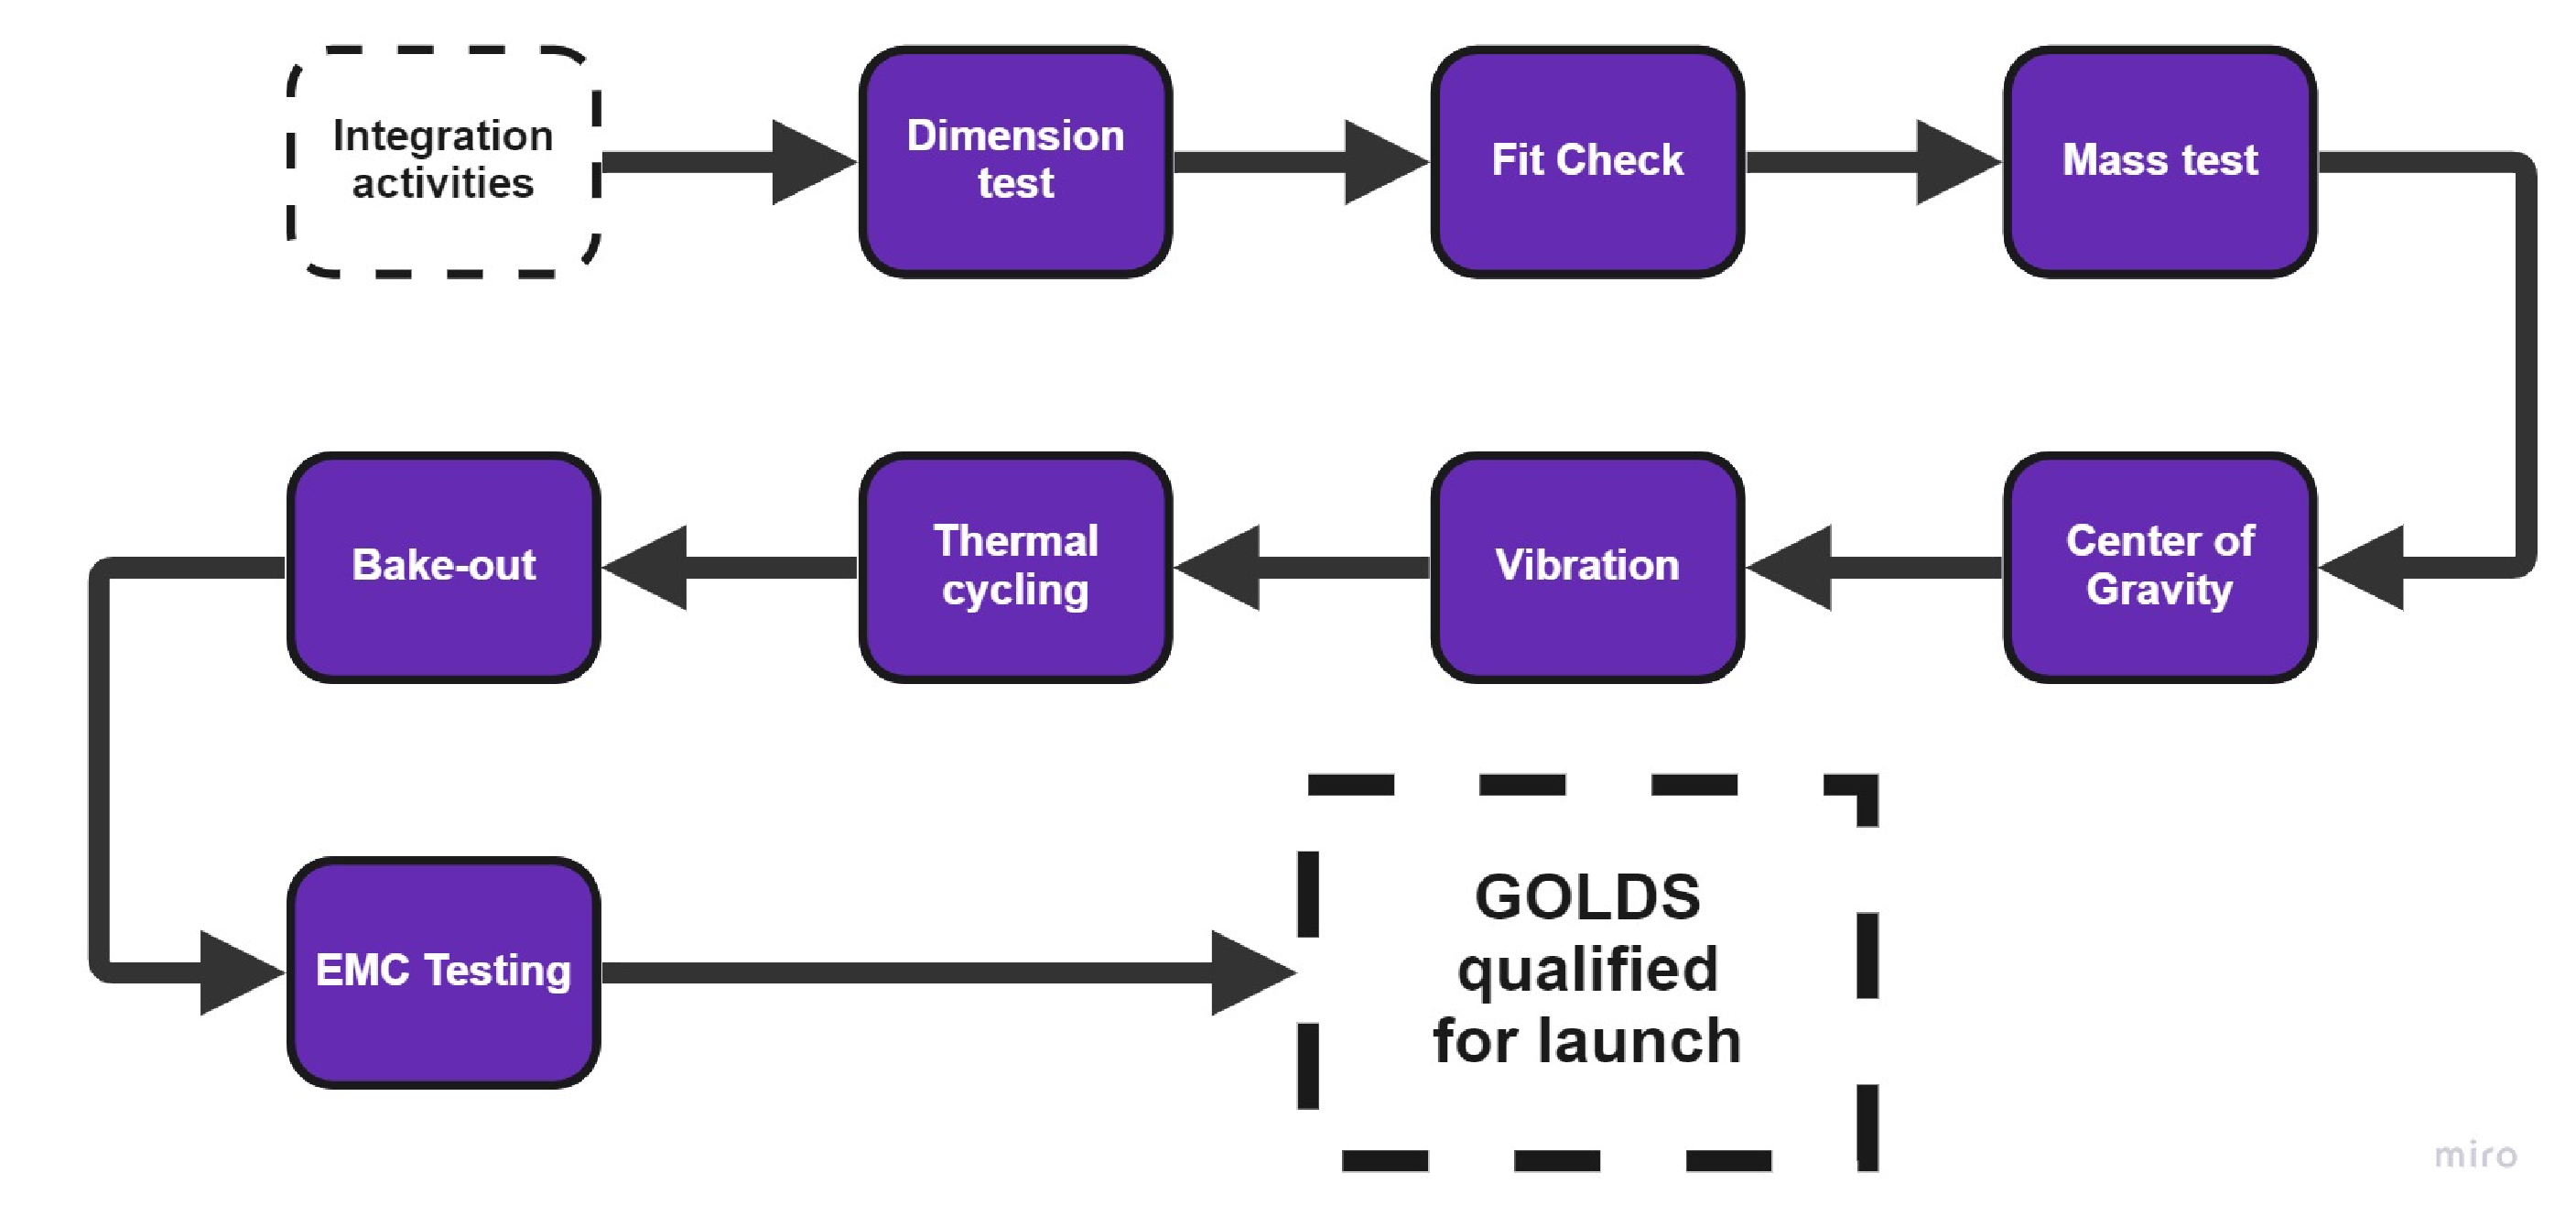
\includegraphics[scale=0.3]{figures/tests_chart.pdf}
    \caption{Test sequence for Radio Occultation.}
    \label{fig:testesequency}
\end{figure}

In the following sections, these tests are described.

%Observation: The vibration tests require the integration of Radio Occultation with the Picosatellite Orbital Deployer (POD), whose option for flight model of POD or identical structure is dictated by the launcher office. The provision of POD is responsibility of the launcher office.

\subsection{Dimensions}

This test checks the main external dimensions of Radio Occultation and aims to prove that its dimensions are appropriate for integration in a standard 2U CubeSat deployer. The dimensional test is validated by measuring with a caliper or micrometer the main external dimensions of Radio Occultation, according to \autoref{fig:fitcheck}. The tolerance is $\pm$0.1 mm in the X, Y, and Z axis. Any measurement out of this range means the CubeSat is not ready for launch.

\begin{figure}[!htb]
    \begin{center}
        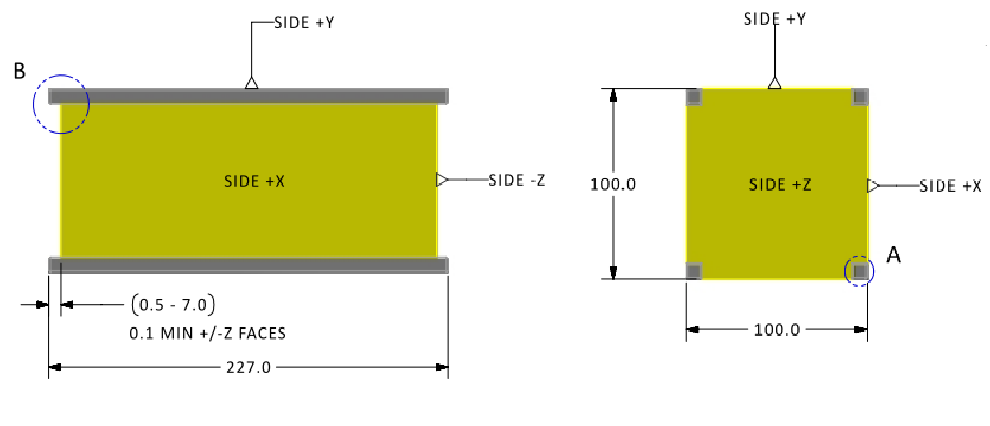
\includegraphics[width=0.9\textwidth]{figures/fit_check.png}
        \caption{Dimensional validation. Adapted from \cite{cds}.}
        \label{fig:fitcheck}
    \end{center}
\end{figure}

\subsection{Fit check}

To assure a proper integration and deployment of the CubeSat, a similar 2U deployer used by the launch is fundamental to verify any additional mechanical interference between these interfaces, as illustrated in \autoref{fig:PODfitcheck}. A smooth sliding through the deployer, the absence of interference, and proper pressing of kill-switches are required for qualification.



\begin{figure}[!htb]
    \begin{center}
        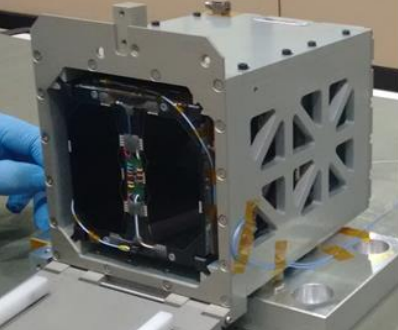
\includegraphics[width=0.4\textwidth]{figures/fit-test.png}
        \caption{Radio Occultation fit check.}
        \label{fig:PODfitcheck}
    \end{center}
\end{figure}


Therefore, this activity lacks a better definition until the launch vehicle and its mandatory deployer are confirmed.

\subsection{Mass}

This test checks the satellite's total mass (without RBF tag), which must be less than 4.00 kg for a 2U CubeSat \cite{cds}. The verification is made with a precision balance. \autoref{fig:mass-verification} exemplifies this process with the CubeSat 1U Radio Occultation.

\begin{figure}[H]
    \begin{center}
        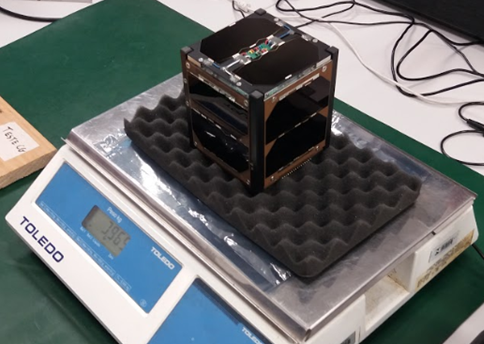
\includegraphics[width=0.7\textwidth]{figures/mass-test.png}
        \caption{Mass verification of Radio Occultation.}
        \label{fig:mass-verification}
    \end{center}
\end{figure}

\subsubsection{Center of Gravity}

This test checks the Center of Gravity (CG) of the satellite and proves if it is within the acceptable range. The CG must be within $\pm$2.0 cm from the geometric center on the X-Axis and Y-Axis, and within $\pm$4.5 cm from the geometric center on the Z-Axis \cite{cds}. To perform this test, a simple test bench with parallel bars is used. To perform the test, the bars are 4.0 cm apart (to test in the X and Y-axis) or 9.0 cm apart (to test the Z-axis), the geometric center of CubeSat is positioned above them, right between the bars. The CubeSat is not going to tip if the CG is within the range. This strategy does not measure the location of CG; however, it does prove that the satellite follows the requirement.

This test was already validated with Radio Occultation, as illustrated in \autoref{fig:cg}, where a caliper is used to verify that the distance between the bars are 4.0 cm.

\begin{figure}[!htb]
    \begin{center}
        \subfigure[$X$ axis.\label{fig:fsat-fm-x-axis}]{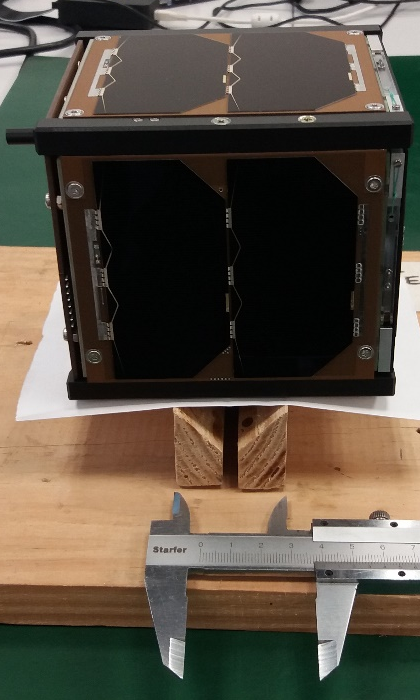
\includegraphics[width=0.2\textwidth]{figures/fsat_fm_x_axis.png}}
        ~
        \subfigure[$Y$ axis.\label{fig:fsat-fm-y-axis}]{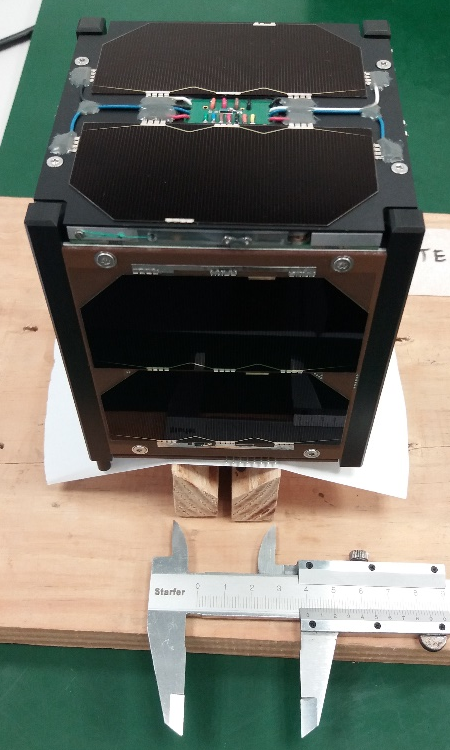
\includegraphics[width=0.2\textwidth]{figures/fsat_fm_y_axis.png}}
        ~
        \subfigure[$Z$ axis.\label{fig:fsat-fm-z-axis}]{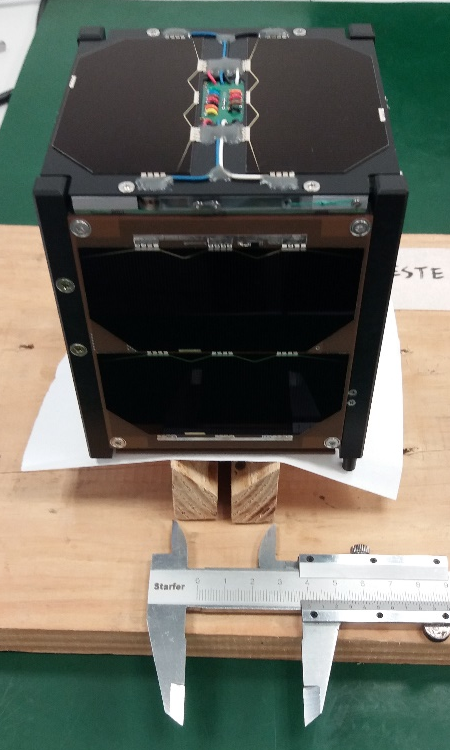
\includegraphics[width=0.2\textwidth]{figures/fsat_fm_z_axis.png}}
        \caption{Center of gravity of Radio Occultation within $\pm$2.0 cm from the geometric center.}
        \label{fig:cg}
    \end{center}
\end{figure}

\subsection{Vibration}

During the launch phase, a significant level of vibration is expected, which can cause failures in the CubeSat. To determine if the CubeSat supports those loads, vibration test are performed. To measure and control the acceleration profile during the dynamic tests, accelerometers are positioned on three external surfaces of the satellite, one on each axis, over areas without solar cells to avoid any damage to them, as illustrated for the case of Radio Occultation in \autoref{fig:fsat-vibration-accel}. After that, the satellite is integrated into a 2U test deployer, and then the deployer is fixed on a shaker, as seen in \autoref{fig:fsat-vibration-accel}.

\begin{figure}[!htb]
    \begin{center}
        \subfigure[Position of the accelerometers.\label{fig:fsat-vibration-accel}]{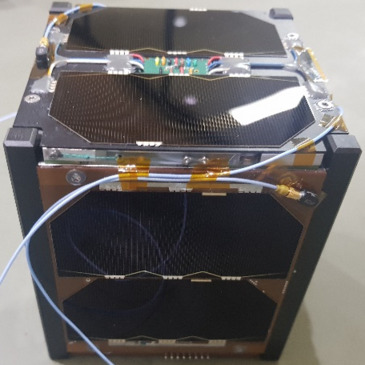
\includegraphics[height=4.5cm]{figures/fsat_fm_accel.jpg}}
        ~
        \subfigure[Shaker.\label{fig:fsat-shaker}]{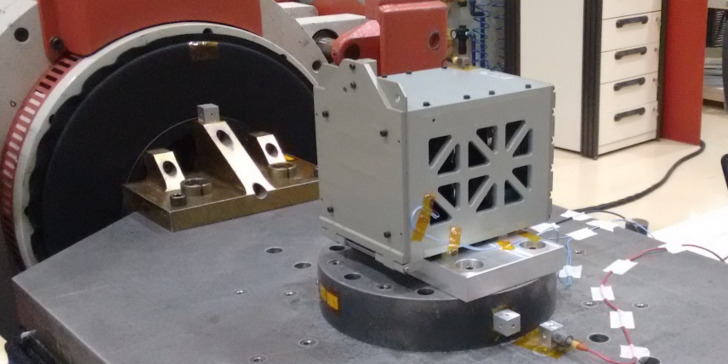
\includegraphics[height=4.5cm]{figures/fsat_fm_shaker.jpg}}
        \caption{Vibration test.}
        \label{fig:vibration-test}
    \end{center}
\end{figure}

The CubeSat is tested entirely off, with RBF pin removed, but with the Kill-Switches pressed by the 2U Test POD, simulating the normal launching condition. The envelope of vibration is determined by the launch vehicle, therefore, this activity lacks a better definition until the launch vehicle is confirmed.

Nevertheless, this test is usually executed for most of the CubeSat missions, so a preliminary set of vibration tests is anticipated in \autoref{fig:vibration_procedure}. This process will be followed until further information from the launch vehicle is provided.

\begin{figure}[!htb]
    \begin{center}
        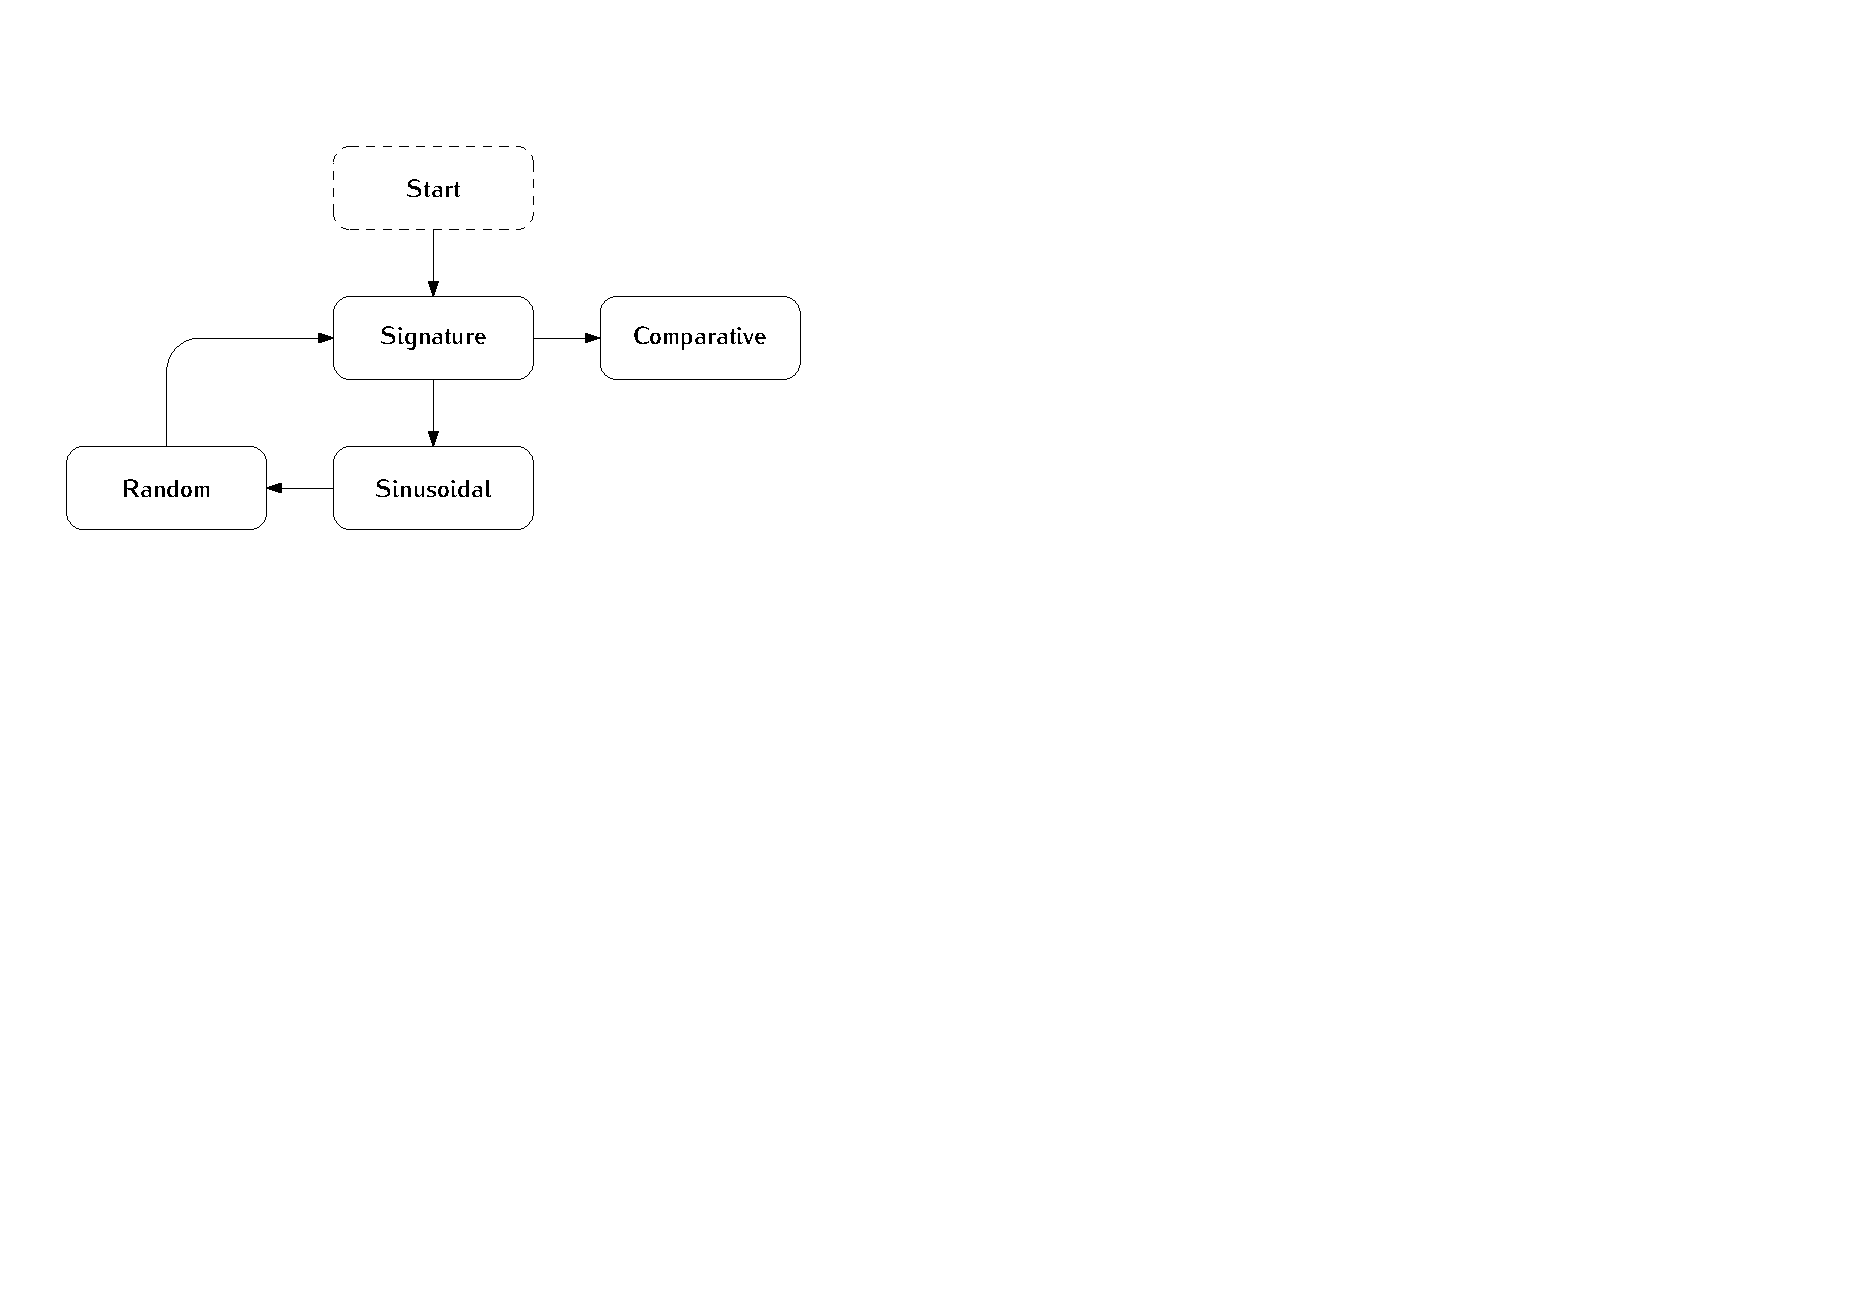
\includegraphics[width=0.6\textwidth]{figures/vibration_procedure.pdf}
        \caption{Sequence of dynamic tests.}
        \label{fig:vibration_procedure}
    \end{center}
\end{figure}

A signature testing should be conducted before and after the tests (sinusoidal and random vibration), in order to identify the presence of significant variations in the dynamic response of the CubeSat, a condition that may represent internal mechanical failures that are non-visible from outside.

For the signature task, \autoref{tab:vibration-test-dynamic-1} presents the specifications.

\begin{table}[!htb]
    \begin{center}
        \begin{tabular}{ll}
            \toprule[1.5pt]
            \textbf{Name}    & \textbf{Parameter}       \\
            \midrule
            Test method      & Sinusoidal sweep testing \\
            Frequency range  & 5 - 2000 Hz              \\
            Vibration level  & 0.25 g                   \\
            Sweep rate       & 2 octaves per minute     \\
            Number of sweeps & 1 (5 - 2000 Hz)          \\
            Test axes        & 3 ($X$, $Y$, $Z$)        \\
            \bottomrule[1.5pt]
        \end{tabular}
        \caption{Resonance survey test (signature).}
        \label{tab:vibration-test-dynamic-1}
    \end{center}
\end{table}

%Regarding the sinusoidal sweeping vibration, Table 3 brings the envelope of the test, and so does Fig. 24 in a graphic format.


\subsubsection{Sinusoidal vibration test}

The sinusoidal vibration test should simulate low-frequency quasi-harmonic excitation of the launch in the order of 5 to 100 Hz. The level of sine sweeping vibration test is listed in Fig. \ref{fig:vibration-sinusoidal-curve} and Table \ref{tab:sinetest}.


\begin{table}[!htb]
    \centering
    \begin{tabular}{C{0.22\textwidth}C{0.22\textwidth}C{0.22\textwidth}C{0.22\textwidth}}
        \toprule[1.5pt]
        \multicolumn{2}{c}{\textbf{Acceptance Test}} & \multicolumn{2}{c}{\textbf{Qualification Test}} \\
        \midrule
        Frequency Range (Hz) & Vibration Amplitude & Frequency Range (Hz) & Vibration Amplitude \\
        \midrule
        5$\sim$8   & 2.33mm(0-p) & 5$\sim$8   & 3.49mm(0-p) \\
        8$\sim$100 & 0.6g        & 8$\sim$100 & 0.9g \\
        \bottomrule[1.5pt]
    \end{tabular}
    \caption{Sinusoidal Sweeping Vibration Test Condition.}
    \label{tab:sinetest}
\end{table}

\begin{figure}[!htb]
    \begin{center}
        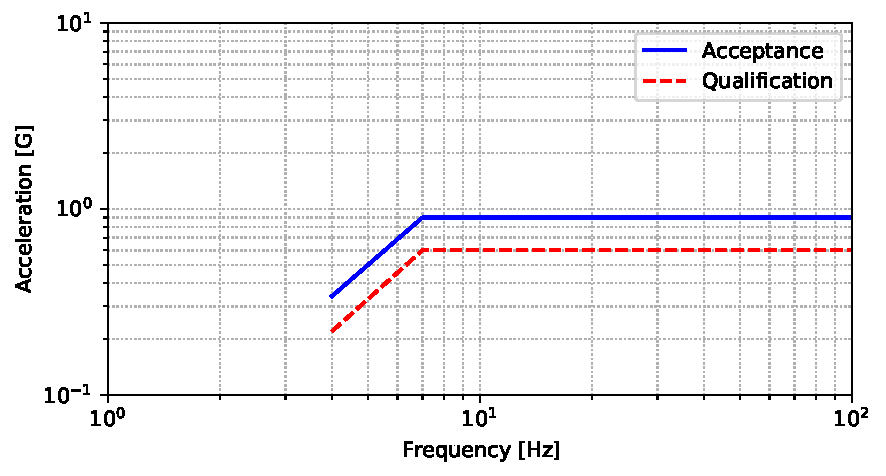
\includegraphics[width=\textwidth]{curves/sine_test.pdf}
        \caption{Sinusoidal sweeping vibration curve.}
        \label{fig:vibration-sinusoidal-curve}
    \end{center}
\end{figure}

The sweeping rates of the acceptance test and qualification tests are 4oct/min and 2oct/min, respectively. The test directions are along three orthogonal axes, and the levels along the three directions are the same. Input amplitude errors do not exceed $\pm 10$\% while frequency error is $\pm2$\% when frequency $>$ 25 Hz or $\pm0.5$ Hz when frequency $\leq$ 25 Hz.

%For the rigidly fixed satellite or SC/adapter assembly, appropriately reducing the input level, controlling the input bending moment at the separation plane will simulate the flight condition more accurately. The bending moment at the SC/LV separation plane is, generally, determined through SC/LV coupled computation or flight data of similar launch vehicles.

%When the satellite carries out sine sweeping test, the bending moment at SC/LV separation plane can be limited through pre-set notching and maximum response control. The satellite notching test scheme is determined through negotiation between the customer and SAST.

\subsubsection{Random vibration}

 This test follows the NASA-STD-7001B standard. This test profile is specified in \autoref{tab:vibration-random} and illustrated in \autoref{fig:vibration-random}. The random vibration is performed by 2 minutes, along each of three orthogonal axes.

\begin{figure}[!htb]
    \begin{center}
        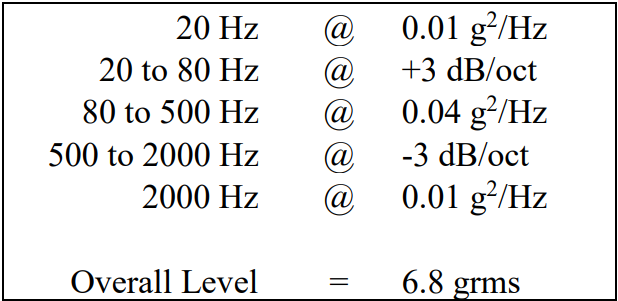
\includegraphics[width=0.6\textwidth]{figures/random-vibration.png}
        \caption{Component Minimum Workmanship Random Vibration Test Levels.}
        \label{tab:vibration-random}
    \end{center}
\end{figure}

\begin{figure}[!htb]
    \begin{center}
        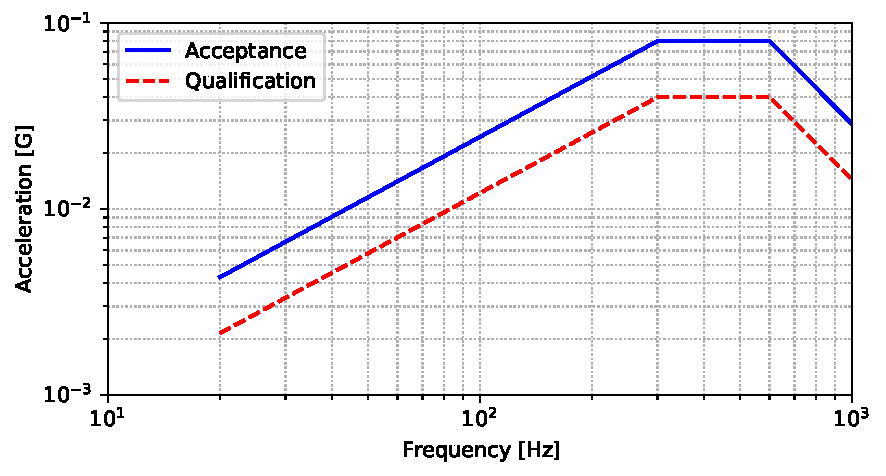
\includegraphics[width=\textwidth]{curves/random_vibration.pdf}
        \caption{Random vibration test.}
        \label{fig:vibration-random}
    \end{center}
\end{figure}

\subsection{Thermal Cycling}

For the thermal tests, thermocouples are attached to different points on the surface of the satellite, including over the solar panels and structure. For example, \autoref{fig:fsat-thermal-test} shows Radio Occultation ready for thermal tests. This test may ruled by the launch vehicle requirements, but until there is no further information about it, the parameters of the tests are summarized in \autoref{tab:thermal_cycling}.

\begin{figure}[!htb]
    \begin{center}
        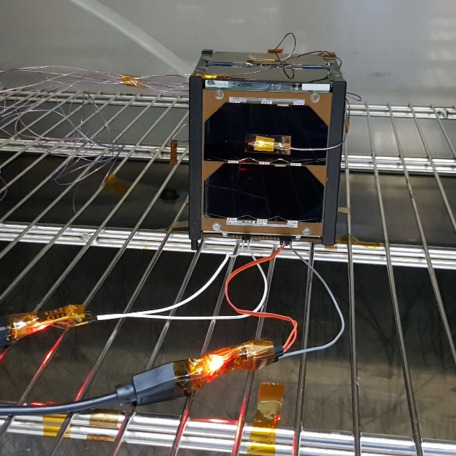
\includegraphics[width=0.4\textwidth]{figures/fsat_fm_thermal_cycling.jpg}
        \caption{Radio Occultation during the thermal cycling (with thermocouples).}
        \label{fig:fsat-thermal-test}
    \end{center}
\end{figure}

\begin{table}[!htb]
    \centering
    \begin{tabular}{ll}
        \toprule[1.5pt]
        \textbf{Parameter} & \textbf{Value} \\
        \midrule
        Number of cycles        & 6 \\
        Minimum temperature     & $T_{min}=-15 ^\circ$C \\
        Maximum temperature     & $T_{max}=+50 ^\circ$C \\
        Duration in $T_{min}$   & 30 min \\
        Duration in $T_{max}$   & 60 min \\
        Heating rate            & 5.5 $^\circ$C/min \\
        Cooling rate            & 3.5$^\circ$C/min \\
        Stabilization criteria  & 1$^\circ$C/10 min \\
        \bottomrule[1.5pt]
	\end{tabular}
    \caption{Parameters for the thermal cycling.}
    \label{tab:thermal_cycling}
\end{table}

\subsection{Bake Out}

Here the CubeSat is exposed to a high temperature in a high vacuum environment during a determined time to stimulate their outgassing to fulfill a requirement established to launch. The Bake-out test requirements usually come from the launch provider, but in the absence of this information, the plan is summarized in Table \ref{tab:bakeout_cycling}. %https://s3vi.ndc.nasa.gov/ssri-kb/static/resources/ICES_2017_102.pdf

\begin{table}[!htb]
    \centering
    \begin{tabular}{ll}
    \toprule[1.5pt]
    \textbf{Parameter} & \textbf{Value} \\
    \midrule
    \multicolumn{2}{c}{Part 1} \\
    \midrule
    Pressure           & <1$\times 10^{-4}$ mbar \\
    Temperature        & 23 $^\circ$C \\
    Duration           & 12 hours \\
    \midrule
    \multicolumn{2}{c}{Part 2} \\
    \midrule
    Pressure           & <1$\times 10^{-4}$ mbar \\
    Temperature        & 60 $^\circ$C \\
    Duration           & 6 hours \\
    \bottomrule[1.5pt]
    \end{tabular}
    \caption{Parameters for the bake out.}
    \label{tab:bakeout_cycling}
\end{table}

\subsection{EMC Testing}


\subsubsection{EMC: Radiation Emission(RE)}
For EMC Radiation Emission test, refer to ECSS-E-ST-20-07C clause 5.4.6. The levels
can be found at ECSS-E-ST-20-07C Annex A. The number of applications shall be one.

\subsubsection{EMC: Conducted Emission (CE)}
For EMC Conducted Emission test, refer to ECSS-E-ST-20-07C clause 5.4.2 The levels
can be found at ECSS-E-ST-20-07C Annex A. The number of applications shall be one.

\subsubsection{EMC: Radiation Susceptibility (RS)}
For EMC Radiation Susceptibility test, refer to ECSS-E-ST-20-07C clause 5.4.11 The
levels can be found at ECSS-E-ST-20-07C Annex A. The number of applications shall be one.

\subsubsection{EMC: Conducted Susceptibility (CS)}
For EMC Conducted Susceptibility test, refer to ECSS-E-ST-20-07C clause 5.4.7 The
levels can be found at ECSS-E-ST-20-07C Annex A. The number of applications shall be one.


%\section{Pre-launch Preparation}

%\begin{enumerate}
%    \item .
%    \item .
%\end{enumerate}

%\subsection{Keys of the Telecommands}

%\begin{enumerate}
%    \item .
%    \item .
%\end{enumerate}

%\subsection{Firmware Upload}

%\begin{enumerate}
%    \item .
%    \item .
%\end{enumerate}

%\subsection{Memory Reset}

%\begin{enumerate}
%    \item .
%    \item .
%\end{enumerate}

%\section{Transport to Launch}

%\subsection{Packing the Satellite}

%\begin{enumerate}
%    \item .
%    \item .
%\end{enumerate}

%\subsection{Unpacking the Satellite}

%\begin{enumerate}
%    \item .
%    \item .
%\end{enumerate}
